\documentclass[]{article}

\usepackage{marginnote}
\usepackage{verbatim}
\usepackage[letterpaper,left=3cm,right=4cm]{geometry}

\usepackage{graphicx}

\usepackage{fancyhdr}
\pagestyle{fancy}

\usepackage[colorlinks=true]{hyperref}
\hypersetup{allcolors={blue}}
\hypersetup{pdftitle={Probability Distribution Workshop}}
\hypersetup{pdfauthor={Paul Glezen}}
\hypersetup{pdfcreator={Latex}}
\hypersetup{pdfkeywords={ISAB, Workshop, Probability, Distributions}}

\setlength{\parindent}{0em}
\setlength{\parskip}{1em}

\title{Probability Distribution Workshop}
\author{Los Angeles County\\ISAB}
\date{}

\begin{document}
\maketitle

\section{Introduction}

This workshop is a review of common probability distributions.
It has two principal goals.

\begin{enumerate}

\item Serve as a review for people that have not studied this material
   for a while.

\item Provide exercise for people to familiarize themselves with their
   Python and R distributions.

\end{enumerate}

The exercises themselves are detailed in \emph{Jupyter notebooks} for 
Python and \emph{R markdown} for R.  This mathematical supplement
serves to provide some theoretical motivation for functions encountered
in the Python and R libraries.

\subsection{Availability}

The source code for this document
along with the Python and R exercises are available from the ISAB
GitHub repository.

\href{https://github.com/lacounty-isab/workshops/tree/master/distributions}{https://github.com/lacounty-isab/workshops/tree/master/distributions}

\subsection{Who are We?}

ISAB (Information Systems Advisory Body) is a subcommittee of the 
CCJCC (Countywide Criminal Justice Coordination Committee)
of Los Angeles County, California.
ISAB is a multi-jurisdictional organization serving the justice
communities within the county. 
The ISAB Data Science Committee (IDSC) addresses data science issues
faced by the community. This article addresses skill development.
It is not intended as an endorsement of any one product
or technology.

More details on ISAB and CCJCC can be found on their websites.

\begin{itemize}
\item[ISAB] \href{http://ccjcc.lacounty.gov/Subcommittees-Task-Forces/Information-Systems-Advisory-Board-ISAB}{http://ccjcc.lacounty.gov/Subcommittees-Task-Forces/Information-Systems-Advisory-Board-ISAB}
\item[CCJCC] \href{http://ccjcc.lacounty.gov/}{http://ccjcc.lacounty.gov/}
\end{itemize}

\section*{Random Variables}

Since this article is not intended to be a foundational exposition on
probability theory, we'll jump right in with a review of random variables.
Recall that an event space $\Omega$ is a set of possible outcomes for an
experiment.  In the case of flipping a single coin, we would have

$$
\Omega = \{\mbox{heads}, \mbox{tails}\}
$$

A random variable $X$ is an assignment from the event space to the real
numbers.

$$
X: \Omega \rightarrow {\rm I\!R}
$$

An example for the case of a coin flip might be

\begin{eqnarray*}
X(\mbox{tails}) & = & 0\\
X(\mbox{heads}) & = & 1
\end{eqnarray*}

A less trivial example would be flipping a coin 100 times where
the outcome is the number of heads.  There are many random varialbes
you could define on this event space.

\begin{itemize}
\item the number of heads,
\item the number of tails,
\item 0 if even number of heads, 1 otherwise,
\item greatest number consecutive heads,
\item number of heads minus number of tails.
\end{itemize}

There are many more examples.  Usually the mapping is straight
forward.  In fact, many times the mapping is so straight forward
that we forget that the event and the random variable are not the
same thing!

The goal of the random variable is to convert the experiment
outcomes from an abstract "set of things" to a set of numbers.
This isn't hard when the set of things naturally maps to a set
of numbers in a useful way.  When it's not so natural, we
sometimes have to go back to the definition the right mapping.
Ultimately the goal is to get a set of number with which we
can analyze the experiment quantitatively.

\section{Distributions}

Once we have a random variable defined for an experiment that
maps outcomes to real numbers, the next question is to ask
how the values of the random variable are likely to be
distributed along the real axis after performing the
experiment many times.  A central concept to answering
this question is the \emph{distribution} or 
\emph{cumulative distribution}.

$$
F_X(t) = P(X \le t)
$$

If we think back to the example in the previous section
of flipping a coin 100 times where the random variable X
represented the number of heads, then $F_X(t)$ represents
the probability that the number of heads is less than or
equal $t$.  Some obvious values are

\begin{eqnarray*}
F_X(-1) & = & 0\\
F_X(100) & = & 1
\end{eqnarray*}

The first equality follows from the fact we can't have a
negative count of the number of heads.  The second
equality follows from the fact that we can't encounter
more than 100 heads if we only flip the coin 100 times.
A graph for all values of $t$ is shown below.

  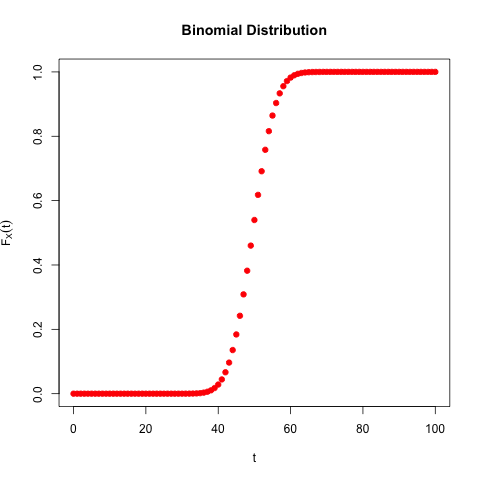
\includegraphics[height=6cm,keepaspectratio]{cdf1.png}

The function $F_X$ is often called the
\emph{cumulative distribution} since it represents the
accumulation of probability as $t$ covers more of the
real axis.  In the figure above for a binomial
cumulative distribution for 100 trials of a fair coin,
we can see that probability of observing less than 40
heads is close to zero.  The probability of observing
less than 60 is close to one.  That tells us that the
most likely scenarios are between 40 and 60.

\subsection{Discrete Densities}

\emph{Discrete distributions} describe experiments where the
random variable takes on discrete values.  These are
often associated with counts.  Their notation will often
be written as $P(X \le n)$ to emphasize the discrete character
of $n$. (Note that $n$ doesn't have to be an integer.)

A \emph{discrete density} $f_X$ corresponding to a discrete
distribution $F_X$ assigns a probability to each discrete value
of the random variable.  If the random variable only takes
integer values, then the density and the distribution
are related in the following ways.

\begin{eqnarray*}
f(n) & = & F(n) - F(n-1)\\
F(n) & = & \sum_{i \le n} f(i)\\
\sum_{i=-\infty}^{\infty} f(i) & = & 1
\end{eqnarray*}

The X subscripts were dropped for brevity; but in general
one writes $F_X$ or $f_X$ to associate the function with
the associated random variable $X$.  This becomes more
important when multiple random variables are considered.

Many useful quantities can be expressed in terms of a density.
First, there is the \emph{mean}.

\begin{equation} \label{discrete_mean}
E[X] = \sum_{i = -\infty}^{\infty} i \cdot f_X(i)
\end{equation}

And the variance.

\begin{equation} \label{discrete_var1}
\mbox{Var}[X] = \sum_{i = -\infty}^{\infty} (i - E(X))^2 \cdot f_X(i)
\end{equation}

A popular alternative expression for the variance can be
obtained by expanding the square.

\begin{eqnarray}
\mbox{Var}[X] & = & \sum_{i=-\infty}^{\infty} (i - E[X])^2 \cdot f_X(i) \nonumber \\
   & = & \sum_{i=-\infty}^{\infty} (i^2 - 2iE[X] + E[X]^2) \cdot f_X(i) \nonumber \\
   & = & \sum_{i=-\infty}^{\infty} i^2 \cdot f_X(i) 
       - 2E[X] \sum_{i=-\infty}^{\infty} i \cdot f_X(i)
       - E[X]^2 \sum_{i=-\infty}^{\infty} f_X(i) \nonumber \\
   & = & E[X^2] - 2E[X] E[X] - E[X]^2 \nonumber \\
   & = & E[X^2] - E[X]^2   \label{discrete_var2}
\end{eqnarray}

This is often expressed in words as ``the mean squared minus the
square of the mean.''  In the special case where the mean is zero,
the variance is equal the mean squared.

The mean is a special cases of a \emph{moments}.
The $n^{\mbox{th}}$ moment is defined as

$$
E[X^n] = \sum_{i = -\infty}^{\infty} i^n \cdot f_X(i)
$$

We've already seen that the first moment is the mean.
The second moment can be used to determine the variance.
Higher moments are not
discussed as often, but they still come in handy.  The
third moment is related to the \emph{skew}, which describes
the degree
to which a distribution is lopsided with respect to its
mean.  The fourth moment is related to the \emph{kurtosis}.  It
describes the extent to which a distribution avoids its mean.

An important tool used in working with distributions is the
\emph{moment generating function}.  For a discrete random
variable, it's defined as

\begin{equation} \label{discrete_mgf}
m_X(t) = E(e^{it}) = \sum_{i=-\infty}^{\infty} e^{it} f_X(i)
\end{equation}

At first glance it looks like way more trouble than it could
possibly be worth.  But moment generating functions turn out
to be important both practically and theoretically.

The theoretical importance derives from analytic function
theory which describes a class of functions that are completely
determined in some neighborhood of a point by the derivatives 
of all orders at the point.  Moment generating functions are
used to show how, in most cases, a distribution is uniquely
determined by the value of all its moments.  This result
is encountered in many proofs to show how a particular
distribution is, in fact, equal to a known distribution.

The practical use is that moment generating functions
often simplify the symbolic calculation of the mean and
variance for many distributions.  The results we need
for the mean and variance are the following.

Given $m_X(t)$ as described in (\ref{discrete_mgf}), the
first and second moments of X are, respectively,

\begin{eqnarray}
E(X) & = & m_X'(0) \label{discrete_mgt_d1} \\
E(X^2) & = & m_X''(0) \label{discrete_mgt_d2}
\end{eqnarray}

It's not immediately obvious how this makes things any
easier.  The examples below will bear it out.

\subsubsection{Binomial Distribution}

We've been using the binomial distribution as an example
for much of the introduction.  Recall that the experiment is that
we perform a sequence of $n$ independent Bernoulli trials, each
of which has probability $p$ of being successful.  The outcome is
the number of successful trials.  Let's consider what the
binomial density looks like.

Let $i$ be the number of successes.  Since $i$ is a count between
zero and $n$, $i$ cannot be less than zero or greater than $n$.  So

$$
p(i) = 0, i \not\in 0, 1, 2, \ldots n
$$

For $i \in 0 \ldots n$ there are $i$ successes and $n-i$ failures.
The probability of such a sequence is $i^p \cdot (n-i)^{(1-p)}$
since each outcome is independent of the one before it.  We then
have to account for the number of positions the $i$ occurrences
could have occurred among the $n$ trials.  There are $n$ ways to
pick the first one.  For each one of these, there are $n-1$ ways
to pick the next one.  This continues until we have picked $i$
times down to $n-i+1$.  This leads to the following expression
with $i$ factors for the $i$ chosen positions.

$$
n \cdot n-1 \cdots n-i+1
$$

But this product distinguishes between the order of the successes.
For example, if the first two are successes, it counts first then
second separately from second and then first.  The order doesn't
matter.  So we divide by the number of permutations of $i$ elements,
which is $i!$: $i$ ways to choose the first one, $i-1$ ways to
choose the second one, down to 1.  So the number of ways we
can choose $i$ elements from $n$ elements without replacement
divided by the number of ways we could have ordered $i$ elements,
we get 

\begin{eqnarray*}
\frac{n(n-1) \cdots (n-i+1)}{i!} & = & \frac{n(n-1) \cdots (n-i+1)}{i!} \cdot
         \frac{n-i}{n-i} \cdot \frac{n-i-1}{n-i-1} \cdots 
         \frac{2}{2} \cdot \frac{1}{1} \\
      & = & \frac{n!}{i! (n-i)!} \\
      & = & {n \choose i}
\end{eqnarray*}

The notation in the last expression is read ``$n$ choose $i$''.

Whew!

So a particular occurrence of $i$ successes and $n-i$
failures occurs with probability $p^i \cdot (1-p)^{n-i}$.
Since there are ${n \choose i}$ ways this can happen, the
probability this can happen in \emph{some way} 
(whichever order, we don't care) is

\begin{equation} \label{binomial_density}
f(i) = {n \choose i} p^i (1-p)^{n-i}, i \in 0, \ldots, n
\end{equation}

This is a probability, the sum of all possible values
should add to one.  Using the binomial formula, we have

\begin{eqnarray*}
\sum_{i=-\infty}^{\infty} f(i) & = & \sum_{i=0}^{n} f(i) \\
   & = & \sum_{i=0}^{n} {n \choose i} p^i (1-p)^{n-i}  \\
   & = & [ p + (1-p) ]^2 \\
   & = & 1^2
\end{eqnarray*}

Great! The probabilities sum to one.  Now let's evaluate
the mean and variance of this distribution.  From
(\ref{discrete_mean}) we have to evaluate

$$
\sum_{i=0}^n i {n \choose i} p^i (1-p)^{n-i}
$$

This is not easy to solve in a closed form.  It's
one of those times where we appeal to the moment generating
function.

\begin{eqnarray*}
m_X(t) & = & E(e^{it}) \\
   & = & \sum_{i=0}^n e^{it} {n \choose i} p^i (1-p)^{(n-i)} \\
   & = & \sum_{i=0}^n {n \choose i} (pe^t)^i (1-p)^{(n-i)} \\
   & = & (pe^t + 1 - p)^n \\
   & = & (pe^t + q)^n
\end{eqnarray*}

In the last step, $1-p$ is replaced with $q$.  We just
remember that $p + q = 1$.  Now
differentiate the moment generating function twice with
respect to $t$.

\begin{eqnarray*}
m_X'(t) & = & n(pe^t + q)^{(n-1)} pe^t \\
m_X''(t) & = & n(n-1)(pe^t + q)^{(n-2)} pe^t pe^t +
          n(pe^t + q)^{(n-1)} pe^t \\
   & = & npe^t(pe^t + q)^{(n-2)}((n-1)pe^t + pe^t + q) \\
   & = & npe^t(pe^t + q)^{(n-2)}(npe^t + q)
\end{eqnarray*}

And evaluate each of the derivatives at $t=0$ for the
required moments.

\begin{eqnarray*}
E(X) & = & m_X'(0) \\
   & = & n(pe^0 + q)^{n-1} pe^0 \\
   & = & n(p+q)^{n-1}p \\
   & = & n1^{n-1}p \\
   & = & np  \\
E(X^2) & = & m_X''(0) \\
   & = & npe^0(pe^0 + q)^{(n-2)}(npe^0 + q) \\
   & = & np(p+q)^{n-2} (np + q) \\
   & = & np (np+q) \\
   & = & (np)^2 + npq
\end{eqnarray*}

The mean is $np$ like we would expect.  For the variance,
substitute these values into (\ref{discrete_var2}).

\begin{eqnarray}
\mbox{Var}(X) & = & E(X^2) - E(X)^2 \nonumber \\
   & = & (np)^2 + npq - (np)^2 \nonumber \\
   & = & npq \label{binomial_var}
\end{eqnarray}

\subsubsection{Poisson Process}

A Poisson process is a special type of counting process.
A counting process is a function $N(t), t \ge 0$ that
only takes non-negative integer values, is non-decreasing,
and $N(0)=0$;
i.e. it represents a count of occurrences over time.  The
Python and R workshops provide graphs of the Poisson
probability mass function.

\begin{equation} \label{poisson_pmf}
f_X(k; \lambda) = e^{-\lambda} \frac{\lambda^k}{k!} 
\quad k = 0, 1, 2, \ldots
\end{equation}

The workshops experiment with $\lambda = 5$.  You get a
PMF curve with a hump near $\lambda$.

\textbf{Mean and Variance}

For the mean and variance we appeal once again to the
moment generation function technique.

\begin{eqnarray*}
m_X(t) & = & E(e^{it}) \\
   & = & \sum_{i=0}^n e^{it} e^{-\lambda} \frac{\lambda^k}{k!} \\
   & = & e^{-\lambda} \sum_{i=0}^n \frac{(e^t \lambda)^i}{i!} \\
   & = & e^{-\lambda} e^{e^t \lambda}
\end{eqnarray*}

Now differentiate the moment generating function twice with
respect to $t$.

\begin{eqnarray*}
m_X'(t) & = & e^{-\lambda} e^{e^t \lambda} e^t \lambda \\
        & = & \lambda e^{(t-\lambda) + \lambda e^t} \\
m_X''(t) & = & \lambda e^{(t-\lambda) + \lambda e^t}(1+\lambda e^t)\end{eqnarray*}

Now evaluate each of the derivatives at $t=0$ for the
required moments.

\begin{eqnarray*}
E(X) & = & m_X'(0) \\
   & = & \lambda e^{(0-\lambda) + \lambda e^0} \\
   & = & \lambda e^0 \\
   & = & \lambda \label{poisson_mean} \\
E(X^2) & = & m_X''(0) \\
   & = & \lambda e^{(0-\lambda) + \lambda e^0}(1+\lambda e^0) \\
   & = & \lambda e^0(1+\lambda) \\
   & = & \lambda + \lambda^2
\end{eqnarray*}

The mean is $\lambda$ like we expect.  For the variance we
substitute these values into (\ref{discrete_var2}).

\begin{eqnarray}
\mbox{Var}(X) & = & E(X^2) - E(X)^2 \nonumber \\
   & = & \lambda + \lambda^2 - \lambda^2 \nonumber \\
   & = & \lambda \label{poisson_var}
\end{eqnarray}

\textbf{Motivation}

The curve looks plausible
enough.  But why this function?  Is it just the most
convenient way to express a curve with a hump in a certain
place?  Or is there something special about the expression
in (\ref{poisson_pmf})?

It turns out that this particular "humped curve" does indeed
have some special properties.  In fact, (\ref{poisson_pmf})
can be derived from four properties.

\begin{enumerate}

\item Non-overlapping intervals are independent.

\item The processes is \emph{stationary}.  That is,
  the probability of an occurrence within time $h$
  from zero is the same as the probability of an occurrence
  within time $t$ to $t + h$, it doesn't depend on $t$.
  In symbols: $P[N(t+h)-N(t)]$ depends only on $h$, not $t$.
  
\item $P[N(t) = 1] = \lambda t + o(t)$

\item $P[N(t) \ge 1] = o(t)$

\end{enumerate}

The symbol $o(t)$ represents any quantity second order or
higher.  Namely,

$$
\lim_{t \rightarrow 0} \frac{o(t)}{t} = 0
$$

If $o(t)$ was analytic (and we're not saying it is), then
its power series representation would only have second
order and above terms (i.e. $o(t) = a_2t^2 + a_3t^3 \ldots$).

\subsection{Continuous Distributions}

\emph{Continuous distributions} describe experiments where
the random variable can take continuous values.  Examples
are time intervals and averages of counts.

A \emph{continuous density} $f_X$ corresponding to a continuous
distribution is related through its integral in a way similar to
how a discrete mass function is related through a sum.

\begin{eqnarray*}
F_X(x) & = & \int_{-\infty}^x f(t) dt \\
f_X(x) & = & \frac{dF(x)}{dx}
\end{eqnarray*}

The analogous formulas for expectation and variance also hold.

\begin{eqnarray}
E[X] & = & \int_{-\infty}^{\infty} xf_X(x) dx \label{cont_mean} \\
\mbox{Var}[X] & = & \int_{-\infty}^{\infty} (E[X] - x)^2 f_X(x) dx \label{cont_var}
\end{eqnarray}

Our friend, the moment generating function, continues to be useful
with continuous random variables.

\begin{equation} \label{cont_mgf}
m_X(t) = E[e^{xt}] = \int_{-\infty}^{\infty} e^{xt} f_X(x) dx
\end{equation}

This is the continuous version of (\ref{discrete_mgf}).

\subsubsection{Normal Distribution}

The granddaddy of all distributions is the \emph{normal distribution}.
It has two parameters: the mean $\mu$ and standard deviation
$\sigma$.  The density function for the normal distribution in one
dimension is given by the following formula.

\begin{equation}
f_X(x; \mu, \sigma) = \frac{1}{\sqrt{2\pi}\sigma}e^{\frac{-(x - \mu)^2}{2\sigma^2}}
\end{equation}

It has the familiar bell-shaped curve centered about the mean.
A common practice is to normalize the random variable through
the transformation

$$
z = \frac{x - \mu}{\sigma}
$$

Then it takes the form

\begin{equation}
f_X(z) = \frac{1}{\sqrt{2\pi}}e^\frac{-z^2}{2}
\end{equation}

The moment generation function is defined in the usual way.

\begin{eqnarray*}
m_X(t) &= &E \left[ e^{tx}\right] \\
  &= &\int_{-\infty}^{\infty} e^{tx} \frac{1}{\sqrt{2\pi}\sigma} 
         e^{-\frac{(x-\mu)^2}{2\sigma^2}} dx \\
  &= &\frac{1}{\sqrt{2\pi} \sigma} \int_{-\infty}^{\infty}
       \exp \left[ -\frac{1}{2} \left( \frac{x-\mu}{\sigma} \right)^2 + tx \right] dx
\end{eqnarray*}

From this point it becomes an exercise in completing the square within
the exponent.

\begin{eqnarray*}
-\frac{1}{2} \frac{(x-\mu)^2}{\sigma^2} + tx & = & \frac{1}{2\sigma^2} \left[
      (x-\mu)^2 - 2tx\sigma^2 \right] \\
   &= &\frac{1}{2\sigma^2} \left[ x^2 - 2x\mu + \mu^2 - 2tx\sigma^2 \right] \\
   &= &\frac{1}{2\sigma^2} \left[ x^2 - 2x(\mu + t\sigma^2) + \mu^2 \right] \\
   &= &\frac{1}{2\sigma^2} \left[ [ x^2 - 2x(\mu + t\sigma^2) + (\mu + t\sigma^2)^2 ]
       - (\mu + t\sigma^2)^2 + \mu^2 \right] \\
   &= &\frac{1}{2\sigma^2} \left[ [x - (\mu + t\sigma^2)]^2
       - \mu^2 + 2\mu t \sigma^2 - t^2 \sigma^4 + \mu^2 \right] \\
   &= &\frac{1}{2} \left[ \frac{x - (\mu + t\sigma^2)}{\sigma} \right]^2
      +\frac{1}{2} \left[ 2\mu t + t^2 \sigma^2 \right]
\end{eqnarray*}

Now if we substitute this exponent expression back into our moment
generating function, we get

\begin{eqnarray}
m_X(t) &= &\frac{1}{\sqrt{2\pi} \sigma} \int_{-\infty}^{\infty} \exp \left[
   \frac{1}{2} \left( \frac{x - (\mu + t\sigma^2)}{\sigma} \right)^2
      +\frac{1}{2} ( 2\mu t + t^2 \sigma^2) \right] dx  \nonumber \\
  &= &\exp \left[ \frac{1}{2} ( 2\mu t + t^2 \sigma^2) \right] \frac{1}{\sqrt{2\pi} \sigma} 
   \int_{-\infty}^{\infty} \exp \left[ \frac{1}{2} 
   \left( \frac{x - (\mu + t\sigma^2)}{\sigma} \right)^2 \right] dx \nonumber \\
  &= & \exp \left[\mu t + \frac{1}{2}t^2 \sigma^2 \right] \label{norm_mgf}
\end{eqnarray}

\subsubsection{Exponential Distribution}

The exponential random variable has a cumulative distribution
function of the form

\begin{equation} \label{exp_cdf}
F_X(x; \lambda) = \left\{ \begin{array}{r@{\quad:\quad}l}
   1 - e^{-\lambda x} & x > 0 \\
   0 & x \le 0
 \end{array} \right.
\end{equation}

where $1/\lambda$ is the expected wait-time of a Poisson processes.
As usual, the density function is the derivative of the CDF.

\begin{equation} \label{exp_density}
f_X(x; \lambda) = \lambda e^{-\lambda x}
\end{equation}

To calculate the mean and variance, we resort once again to the
moment generating function.

\begin{eqnarray*}
m_X(t) & = & E[e^{xt}] \\
   & = & \int_0^{\infty} e^{xt} \lambda e^{-x \lambda} dx \\
   & = & \lambda \int_0^{\infty} e^{-x(\lambda - t)} dx \\
   & = & \left. \lambda \cdot \frac{-1}{\lambda - t} e^{-x(\lambda - t)}
      \right|_{x=0}^{x=\infty} \\
   & = & \frac{-\lambda}{\lambda - t} (0 - 1) \\
   & = & \frac{\lambda}{\lambda - t}
\end{eqnarray*}

Note the definite integral only converges for $\lambda - t > 0$.
This is fine for our needs since we intend to evaluate the moment
generating function close to zero for its derivatives at zero.

Now differentiate the moment generating function twice with
respect to $t$.

\begin{eqnarray*}
m_X'(t) & = & \lambda(\lambda - t)^{-2}  \\
m_X''(t) & = & \lambda (-2)(\lambda - t)^{-3}(-1) \\
   & = & \frac{2 \lambda}{(\lambda - t)^3}
\end{eqnarray*}

Now evaluate each of the derivatives at $t=0$ for the
required moments.

\begin{eqnarray*}
E(X) & = & m_X'(0) \\
   & = & \frac{\lambda}{\lambda^2} \\
   & = & \frac{1}{\lambda} \label{expon_mean} \\
E(X^2) & = & m_X''(0) \\
   & = & \frac{2 \lambda}{\lambda^3} \\
   & = & \frac{2}{\lambda^2}
\end{eqnarray*}

The mean is $1 / \lambda$.  For the variance we
substitute these values into (\ref{discrete_var2}).

\begin{eqnarray}
\mbox{Var}(X) & = & E(X^2) - E(X)^2 \nonumber \\
   & = & \frac{2}{\lambda^2} - \frac{1}{\lambda^2} \nonumber \\
   & = & \frac{1}{\lambda^2} \label{poisson_var}
\end{eqnarray}

It turns out the first and second moments are not difficult
to derive directly from their integral formulas.

\begin{eqnarray*}
E[X] & = & \int_0^{\infty} x \lambda e^{-\lambda x} dx \\
E[X^2] & = & \int_0^{\infty} x^2 \lambda e^{-\lambda x} dx
\end{eqnarray*}

It's a straight forward pair of calculations using integration
by parts. But moment generating functions still save a little
bit of work.

\end{document}